%\documentclass{aa}
\documentclass[twocolumn,iop]{openjournal}

\usepackage{natbib}
\bibpunct{(}{)}{;}{a}{}{,} 
\usepackage{graphicx}   
\usepackage{txfonts}
\usepackage[colorlinks=true,allcolors=cyan]{hyperref}

\newcommand{\MSUN}{{\rm M}_\odot}
\newcommand{\mpch}{\>h^{-1}{\rm {Mpc}}}

\begin{document}

\journalinfo{The Open Journal of Astrophysics}
\submitted{submitted}

\shorttitle{haloes, galaxies \& X-ray}
\shortauthors{J. Comparat et al.}
\title{Connecting haloes and galaxies to their X-ray emissions with an empirical model of hot gas and active galactic nuclei} 

\author{Johan Comparat$^{1}$   }
%\author{Andrea Merloni$^{1}$    }

\affiliation{$^{1}$Max-Planck-Institut f\"{u}r extraterrestrische Physik (MPE), Gie{\ss}enbachstra{\ss}e 1, D-85748 Garching bei M\"unchen, Germany}

\thanks{$^\star$ E-mail: \nolinkurl{comparat@mpe.mpg.de}}
    
\date{\today}

\begin{abstract}
This article presents the construction and validation of an X-ray empirical model applied to simulated haloes and the galaxies therein. 

\end{abstract}


\keywords{Large-scale structure, X-ray, galaxies}
\maketitle

%%%%%%%%%%%%%%%%% BODY OF PAPER %%%%%%%%%%%%%%%%%%
%
%
% INTRO
%
%
\section{Introduction}
The SRG/eROSITA telescope \citep{PredehlAndritschkeArefiev_2021A&A...647A...1P,SunyaevArefievBabyshkin_2021A&A...656A.132S} gathered soft X-ray photons over half of the sky providing, among other, a new comprehensive view of the extra-galactic large scale structure observed in X-rays \citep[][, C25 hereafter]{ComparatMerloniPonti_2025arXiv250319796C}.  
In this article, we focus on upgrading the active galactic nuclei model from \citet{ComparatMerloniSalvato_2019MNRAS.487.2005C, ComparatLuoMerloni_2023A&A...673A.122C} and the hot gas model from \citet{ComparatEckertFinoguenov_2020OJAp....3E..13C, SeppiComparatBulbul_2022A&A...665A..78S}. 

\section{Light cone description}
\label{sec:light:cone}

We use the Uchuu simulation \citep{IshiyamaPradaKlypin_2021MNRAS.506.4210I} and the UniverseMachine model \citep{BehrooziWechslerHearin_2019MNRAS.488.3143B, AungNagaiKlypin_2023MNRAS.519.1648A}. 
The DM-only simulation is made of 12 800$^3$ particles in a cube of length 2$h^{-1}$Gpc, corresponding to particles with a mass of $3.27\times10^8h^{-1}$M$_\odot$. 
We create a full sky light up to redshift $z\sim6$ cone by replicating the box (8x8x8 times) using its periodic boundary condition following \citet{ComparatEckertFinoguenov_2020OJAp....3E..13C}. 
We use 31 snapshots to create shells in the light cone. They are at redshifts 0.00, 
0.02, 
0.05, 
0.09, 
0.14, 
0.19, 
0.25, 
0.30, 
0.36, 
0.43, 
0.49, 
0.56, 
0.63, 
0.70, 
0.78, 
0.86, 
0.94, 
1.03, 
1.12, 
1.22, 
1.32, 
1.43, 
1.54, 
1.65, 
1.77, 
1.90, 
2.03, 
2.17, 
2.31, 
2.46, 
2.62, 
2.78, 
2.95, 
3.13, 
3.32, 
3.61, 
3.93, 
4.27, 
4.63, 
5.15, 
5.73. 

\subsection{Foregrounds and backgrounds}
We use the same model for the diffuse and resolved foreground and the diffuse background as  \citet{ComparatEckertFinoguenov_2020OJAp....3E..13C, SeppiComparatBulbul_2022A&A...665A..78S}. 
We re-generate events 
%The files names 'glist.fits' 
%Create 1:1 correspondence with halo files ? Then use the M500c from rockstar ! Does not work, would need to rerun the halo light cone. Likely some missing entries.

%\subsection{Status}

\clearpage
\section{X-ray prediction for the hot gas}

\begin{verbatim}
t_sim_gal['upid']==-1)&(t_sim_gal['Mvir']>=5e11)
M500c>1e11
\end{verbatim}
The virial mass are converted to 500c with the \citet{IshiyamaPradaKlypin_2021MNRAS.506.4210I} mass concentration relation (directly calibrated on Uchuu). 

\subsection{luminosity and temperature}

We take a different approach from \citet{ComparatEckertFinoguenov_2020OJAp....3E..13C} where the scaling relation (and its scatter) is predicted from the covariance matrix. 
We use the best-fit scaling relation between halo mass and soft X-ray luminosity obtained by \citet[][sample 10.5]{ComparatMerloniPonti_2025arXiv250319796C}
\begin{equation}
\log_{10}(L_X E(z)^{-2}\; [erg\; s^{-1}]) = 44.7 + 1.61 (\log_{10}(M_{500c}/M_\odot)-15)    
\end{equation}
with a scatter of $\sigma_{L_X}=$0.3. 
The parameters of the scaling relation can easily be changed giving more flexibility to the model. 
The scaling relation obtained is shown in Fig. \ref{fig:scaling:mass:luminosity}. 
It agrees well with stacking experiments at low halo masses \citep{ZhangComparatPonti_2024A&A...690A.268Z}, in the group regime \citep{PopessoMariniDolag_2024arXiv241117120P}. 
It is in good agreement with observations reported in the literature \citep{LovisariReiprichSchellenberger_2015A&A...573A.118L, LovisariSchellenbergerSereno_2020ApJ...892..102L, MantzAllenMorris_2016MNRAS.456.4020M,AdamiGilesKoulouridis_2018A&A...620A...5A,SchellenbergerReiprich_2017MNRAS.469.3738S, BulbulChiuMohr_2019ApJ...871...50B, LiuBulbulGhirardini_2022A&A...661A...2L,BulbulLiuKluge_2024A&A...685A.106B}.

\begin{figure}
    \centering
    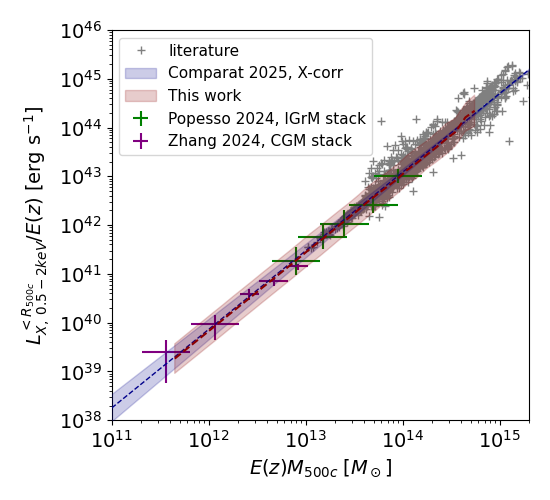
\includegraphics[width=0.95\linewidth]{figures_GAS/M500c_LX.png}
    \caption{Scaling relation between dark matter halo mass (500c) and X-ray luminosity in the 0.5-2 keV band of the mock catalog (red shaded area and red dashed line). 
    It is made using a light cone shell around redshift of z=0.3. 
    It is by construction in agreement with the recent stacking and cross-correlation analysis of \citet[][blue dashes and shaded area]{ComparatMerloniPonti_2025arXiv250319796C}. 
    It agrees well with stacking experiments at low halo masses \citep[][in purple]{ZhangComparatPonti_2024A&A...690A.268Z}, in the group regime \citep[][in green]{PopessoMariniDolag_2024arXiv241117120P} and with the variety of literature measurements for individual groups and clusters \citep[][in grey crosses]{LovisariReiprichSchellenberger_2015A&A...573A.118L, LovisariSchellenbergerSereno_2020ApJ...892..102L, MantzAllenMorris_2016MNRAS.456.4020M,AdamiGilesKoulouridis_2018A&A...620A...5A,SchellenbergerReiprich_2017MNRAS.469.3738S, BulbulChiuMohr_2019ApJ...871...50B, LiuBulbulGhirardini_2022A&A...661A...2L,BulbulLiuKluge_2024A&A...685A.106B}. }
    \label{fig:scaling:mass:luminosity}
\end{figure}

The stellar mass is not used like in \citet{SeppiComparatBulbul_2022A&A...665A..78S} to correct the scaling relation to extend to lower halo masses. In this approach, we predict the relation between stellar mass and X-ray luminosity. We compare the obtained predicted relation to \citet{AndersonGaspariWhite_2015MNRAS.449.3806A} and \citet{ZhangComparatPonti_2024A&A...690A.268Z}. The comparison shows excellent agreement, see Fig. \ref{fig:MsLX}.

\begin{figure}
    \centering
    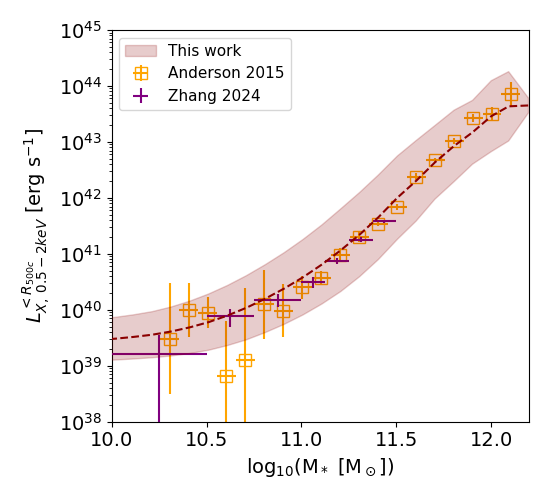
\includegraphics[width=0.95\linewidth]{figures_GAS/Ms_LX.png}
    \caption{Scaling relation between stellar mass and luminosity in the 0.5-2 keV band. It is made using a light cone shell around redshift of z=0.3. The stellar mass is that predicted by the UniverseMachine model independently of the X-ray luminosity. The red dashes and contours is a prediction of the model, which is in excellent agreement with observations from \citet[][in orange]{AndersonGaspariWhite_2015MNRAS.449.3806A} and \citet[][in purple]{ZhangComparatPonti_2024A&A...690A.268Z}.
}
    \label{fig:MsLX}
\end{figure}

For the temperature, we use 
\begin{equation}
\log_{10}(kT\;  E(z)^{-2/3} [keV]) = 0.6 \log_{10}(M_{500c}/M_\odot) - 8
\end{equation}
with a scatter of $\sigma_{kT}=$0.2.
The covariance between the two is  
\begin{verbatim}
[[sigma_kT**2, rho*sigma_kT*sigma_LX ],
[rho*sigma_kT*sigma_LX, sigma_LX**2]]
\end{verbatim}
with $\rho=$0.95. 
We draw a normal random variable from this matrix to add correlated scatter in the observables. 
Future improvement include using the complete mass dependent covariance matrix predicted by hydrodynamical simulations (e.g. Flamingo, Jamal et al. in prep). 
The scaling relation obtained is shown in Fig. \ref{fig:scaling:mass:temperature}.
This line is in good agreement with observations of galaxy groups and clusters \citep{LovisariReiprichSchellenberger_2015A&A...573A.118L, MantzAllenMorris_2016MNRAS.456.4020M, AdamiGilesKoulouridis_2018A&A...620A...5A,BulbulChiuMohr_2019ApJ...871...50B,LovisariSchellenbergerSereno_2020ApJ...892..102L}, with the stacked groups from Toptun et al. in submitted and with the measurement of our own Milky Way from \citep{PontiZhengLocatelli_2023A&A...674A.195P}.

\begin{figure}
    \centering
    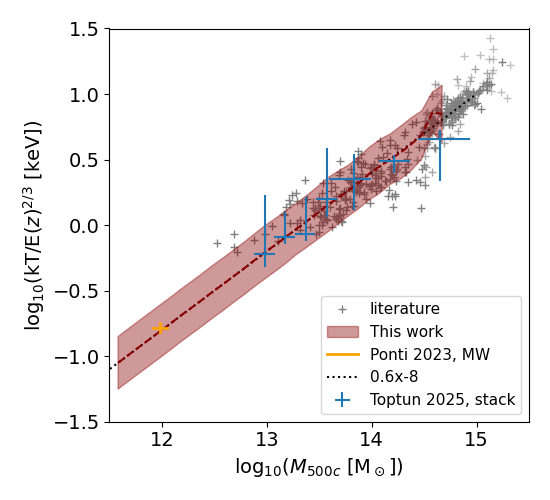
\includegraphics[width=0.95\linewidth]{figures_GAS/M500-kt.png}
%    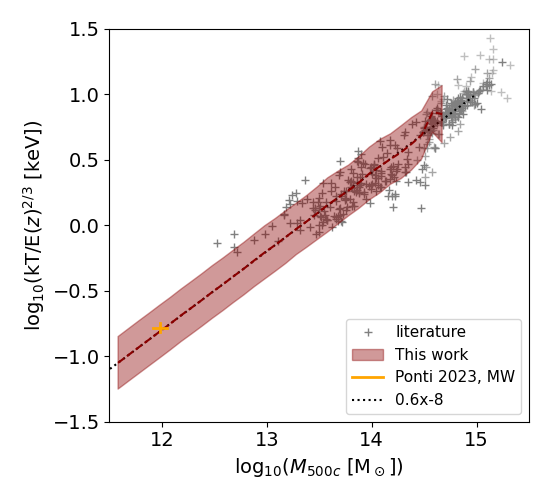
\includegraphics[width=0.95\linewidth]{figures_GAS/M500-kt-noTT.png}
    \caption{Scaling relation between dark matter halo mass (500c) and temperature of the mock catalog (red shaded area and red dashed line). 
    It is made using a light cone shell around redshift of z=0.3. 
    The model prediction is in good agreement with observations of galaxy groups and clusters \citep{LovisariReiprichSchellenberger_2015A&A...573A.118L, MantzAllenMorris_2016MNRAS.456.4020M, AdamiGilesKoulouridis_2018A&A...620A...5A,BulbulChiuMohr_2019ApJ...871...50B,LovisariSchellenbergerSereno_2020ApJ...892..102L}, with the stacked groups from Toptun et al. in submitted and with the measurement of our own Milky Way from \citep{PontiZhengLocatelli_2023A&A...674A.195P}.
}
    \label{fig:scaling:mass:temperature}
\end{figure}



We compute K-correction on a fine grid of redshift and temperature. With that we convert the intrinsic luminosity into an unabsorbed observed flux. Finally, we add absorption using the Nh4PI tabulated skymap \citep{HI4PICollaborationBenBekhtiFloer_2016A&A...594A.116H}. The absorption is tabulated for three temperatures: 0.5, 1 and 2keV. For haloes hotter than 1.5keV, we use the 2keV approximation, for the ones in the range 0.7 to 1.5 keV the 1keV approximation. and the cooler ones with the 0.5 keV approximation. 

The obtained logN-logS (unabsorbed 0.5-2 keV flux) is somewhat bright but its shape follows that of observations (Fig. \ref{fig:logNlogS}). The mock is brighter than observations. This feature was addressed previously by using a hydrostatic mass bias value of 0.8. 
In this iteration, we prefer to avoid adding more parameters since we are interested in the lower mass range where that bias is not applicable due to differences in the measurement procedures. 

\begin{figure}
    \centering
    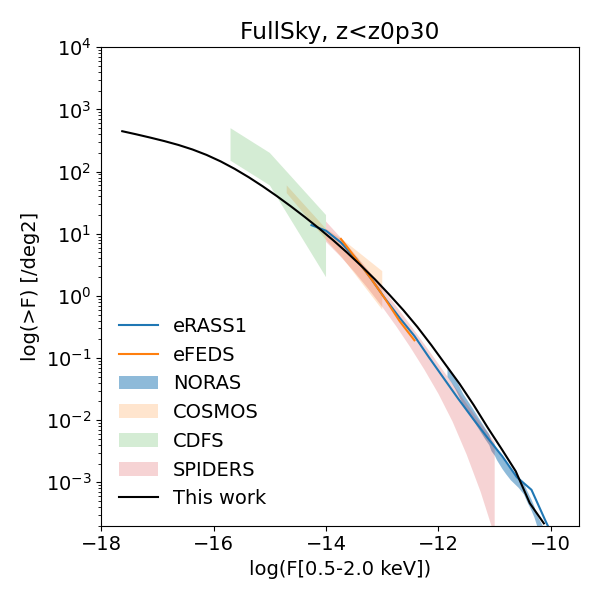
\includegraphics[width=0.8\linewidth]{figures_GAS/FullSky_zlt_z0p30_logNlogS.png}
    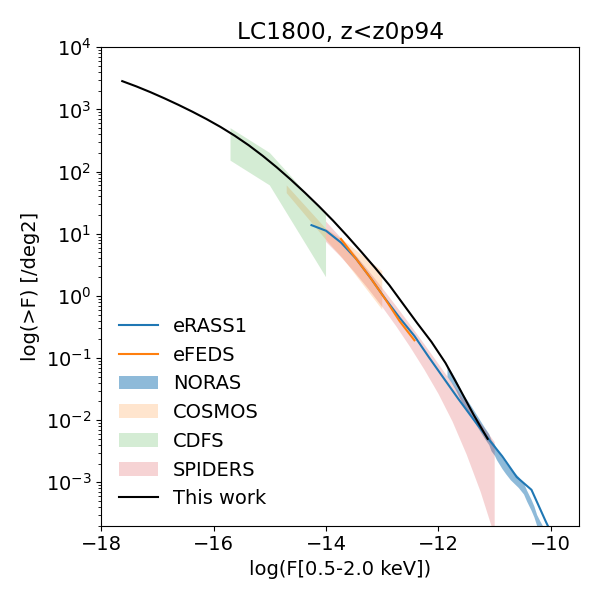
\includegraphics[width=0.8\linewidth]{figures_GAS/LC1800_zlt_z0p94_logNlogS.png}
    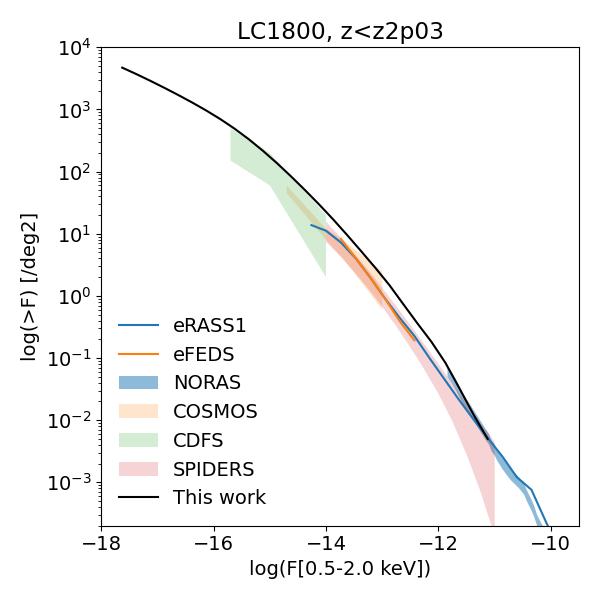
\includegraphics[width=0.8\linewidth]{figures_GAS/LC1800_zlt_z2p03_logNlogS.png}
    \caption{logNlogS. Number density of sources brighter than and observed flux in the 0.5-2 keV band. }
    \label{fig:logNlogS}
\end{figure}

\subsection{X-ray profiles}

We use the method of \citet{ComparatEckertFinoguenov_2020OJAp....3E..13C} to create a library of profile. It represents the diversity of exiting profile shapes encountered in observations. 
The profile shapes are randomly assigned to haloes. 

From \citet{SandersBaharBulbul_2025A&A...695A.160S}, we extract a distribution of ellipticities in four broad bins to obtain the relative frequencies of ellipticities in observations for the S2 volume-limited sample from \citet{SeppiComparatGhirardini_2024A&A...686A.196S}. 
The number of ellipticity values one may use directly scales with the number of images one has to generate. 
In \citet{ComparatEckertFinoguenov_2020OJAp....3E..13C, SeppiComparatBulbul_2022A&A...665A..78S}, we created an image for each source, which was heavy in disk usage and and was proven not to be a key information to model the selection function \citep{SeppiComparatBulbul_2022A&A...665A..78S, ClercComparatSeppi_2024A&A...687A.238C}. 
So we take here a path where less images are created. We sample 2,796 profiles and 4 ellipticities for each redshift shell (22), totaling 246,048 tabulated images representing hot gas profiles up to redshift 1.5.

The ellipticities (denoted $\epsilon$) take four discrete values: [0.55, 0.65, 0.75, 0.85] with fractions of [0.22, 0.30, 0.25, 0.23] representing the fraction of clusters with a given ellipticity value. 


The ellipticity of the images simulated is set at 0.75, the average of the eRASS:1 cluster ellipticities (Sanders et al. 2025).

\subsection*{Event generation}

We re-cast the simput files into the eROSITA sky tiles and merge them to make a single simput per source type in each field. 
Given the mean exposure time of the field, a flux cut is applied to only simulate sources that will generate photons. 
Indeed, image simulations are more intensive, so one should strive for efficiency instead of looping over all haloes and finding out that they emit no events in the time laps simulated. 

We use a synthetic eRASS:8 attitude file to generate a superset of events (containing the observed eRASS:1 or eRASS:5 GTI). For every selection function exercise, the event files are then tailored (GTI filtering) for the specific need. 
Fig. \ref{fig:events:hotgas} illustrates the generated events for the hot haloes. 

\begin{figure}
    \centering
    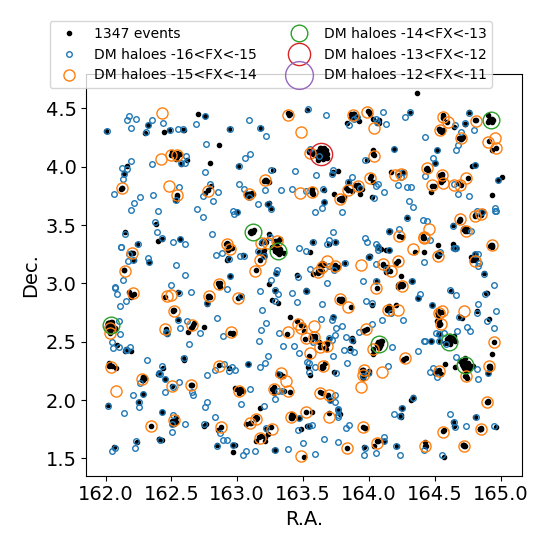
\includegraphics[width=0.95\linewidth]{figures_GAS/ra-dec-hotgas-events.png}
    \caption{Simulated events for the sky tile number 164087. Haloes are split as a function of their total flux (within 2 times $R_{500c}$, the boundary of the simulated image).}
    \label{fig:events:hotgas}
\end{figure}


\clearpage
\section{AGN model}

We use the parametrization from \citet{ComparatMerloniSalvato_2019MNRAS.487.2005C} and \citet{LiuMerloniComparat_2022A&A...661A..27L} with the best combination of parameters found in \citet{ComparatLuoMerloni_2023A&A...673A.122C}. 
The scatter in the abundance matching relation between stellar mass and hard X-ray luminosity function from \citet{AirdCoilGeorgakakis_2015MNRAS.451.1892A} is $\sigma_{AGN}=0.8$ and the satellite fraction is set at $f_{sat}=8\%$. 
The obscuration model is as in \citet{ComparatMerloniSalvato_2019MNRAS.487.2005C}. 

The specific accretion rate distribution (SAR), defined by
\begin{equation}
\lambda_{SAR}=\frac{L^{\rm 2-10\; keV}_X}{M^*},    
\end{equation}
is shown in Fig. \ref{fig:AGN:LSAR}. 
It directly reflects the scatter in the abundance matching relation. 
So, by construction, this model can not recover the double power-law behavior observed, in particular at the high SAR end, see observations from \citet{GeorgakakisAirdSchulze_2017MNRAS.471.1976G, AirdCoilGeorgakakis2018MNRAS.474.1225A}. 
The model agrees fairly well with the observations in the range 30 to 33.

\begin{figure}
    \centering
    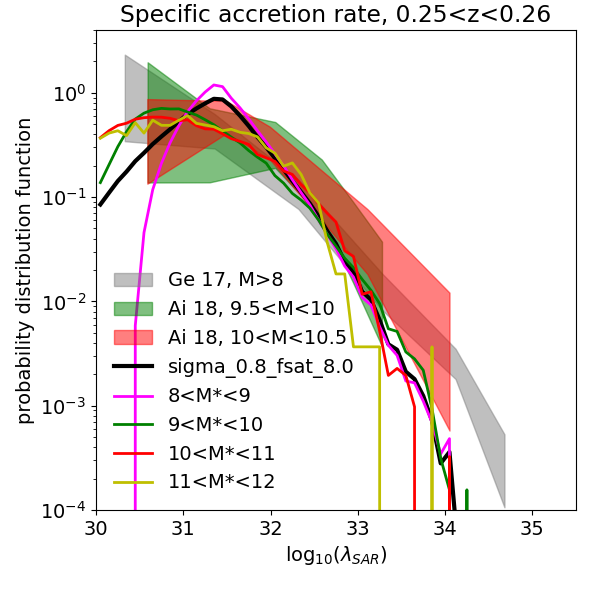
\includegraphics[width=0.95\linewidth]{figures_AGN/LSAR_z025.png}
    %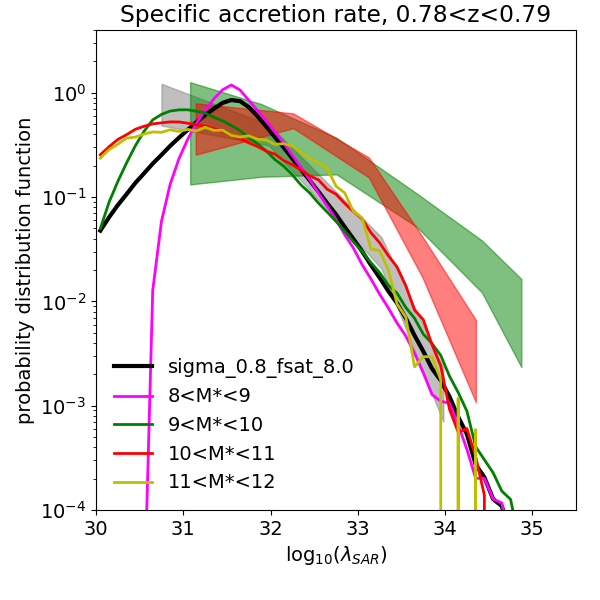
\includegraphics[width=0.45\linewidth]{figures_AGN/LSAR_z075.png}
    %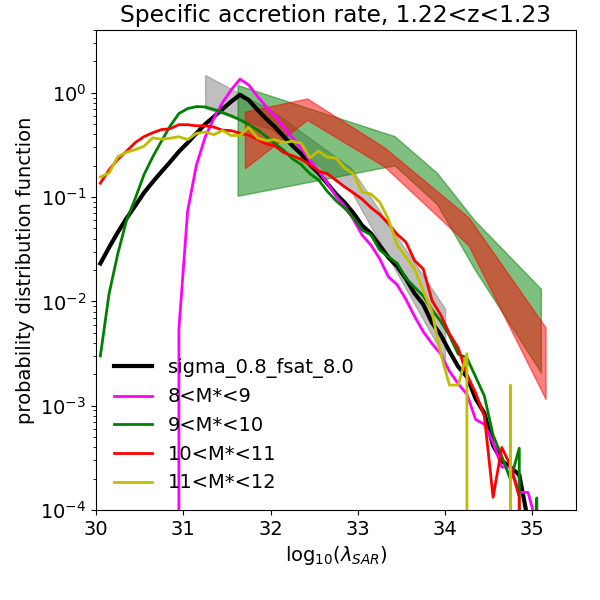
\includegraphics[width=0.45\linewidth]{figures_AGN/LSAR_z125.png}
    \caption{Distribution of specific accretion rate at z=0.25. 
    The model prediction is shown (with colored solid lines) for four stellar mass bins (8, 9, 10, 11, 12).
    It is in fair agreement with observations (shaded areas) from \citet[][Ge17]{GeorgakakisAirdSchulze_2017MNRAS.471.1976G}, \citet[][Ai18]{AirdCoilGeorgakakis2018MNRAS.474.1225A}
    }
    \label{fig:AGN:LSAR}
\end{figure}

The duty cycle obtained is illustrated in Fig. \ref{fig:AGN:duty:cycle}. It follows well observations from \citet{GeorgakakisAirdSchulze_2017MNRAS.471.1976G,ShiRiekeDonley_2008ApJ...688..794S,GeorgakakisCoilWillmer_2011MNRAS.418.2590G}.

\begin{figure}
    \centering
    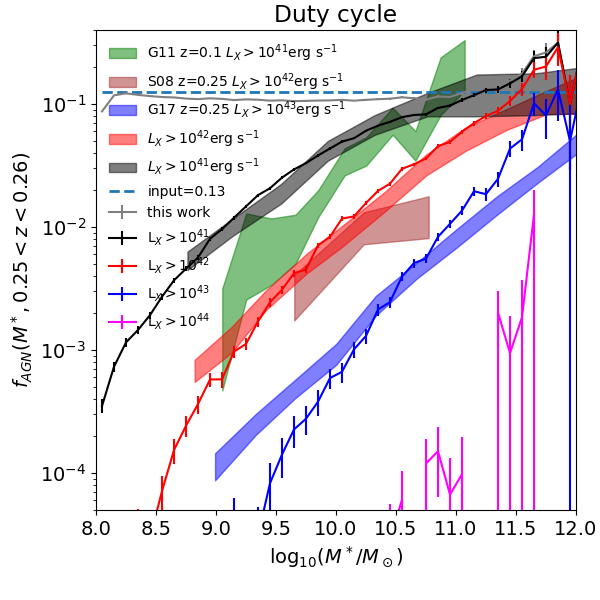
\includegraphics[width=0.95\linewidth]{figures_AGN/DC_z025.png}
    %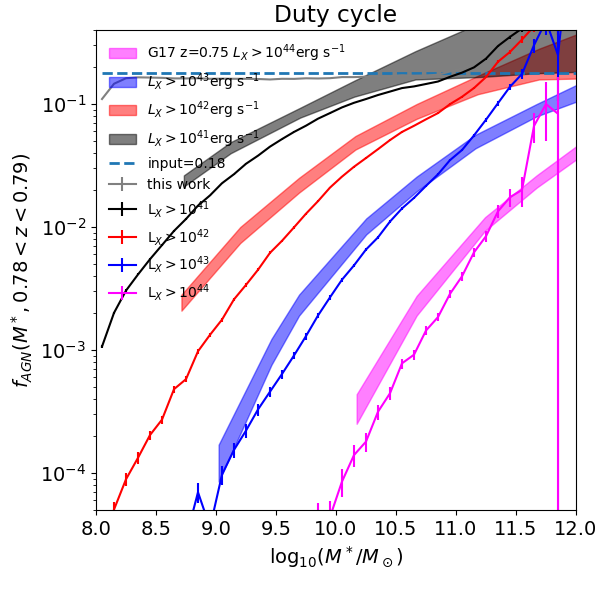
\includegraphics[width=0.45\linewidth]{figures_AGN/DC_z075.png}
    %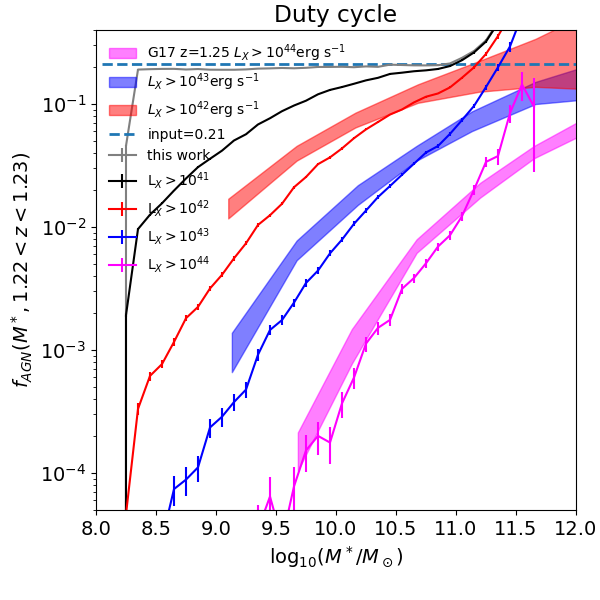
\includegraphics[width=0.45\linewidth]{figures_AGN/DC_z125.png}
    \caption{Duty cycle at z=0.25. Fraction of galaxies with a model active galactic nucleus as a function of stellar mass, provided an input maximum duty cycle of 11\% taken from \citep{GeorgakakisAirdSchulze_2017MNRAS.471.1976G}. 
    The model prediction is shown (with colored solid lines with uncertainties) for four hard X-ray (2-10 keV) luminosity thresholds (41, 42, 43, 44) and the complete sample (grey).
    It is in fair agreement with observations (shaded areas) from \citet[][Ge17]{GeorgakakisAirdSchulze_2017MNRAS.471.1976G}, \citet[][S08]{ShiRiekeDonley_2008ApJ...688..794S}, \citet[][G11]{GeorgakakisCoilWillmer_2011MNRAS.418.2590G}.
    }
    \label{fig:AGN:duty:cycle}
\end{figure}

The obtained stellar mass function of galaxies hosting AGN is shown in Fig. \ref{fig:AGN:SMF}. The shape of the host galaxy stellar mass function is in fair agreement with the model from \citet{BongiornoSchulzeMerloni_2016A&A...588A..78B}.

\begin{figure}
    \centering
    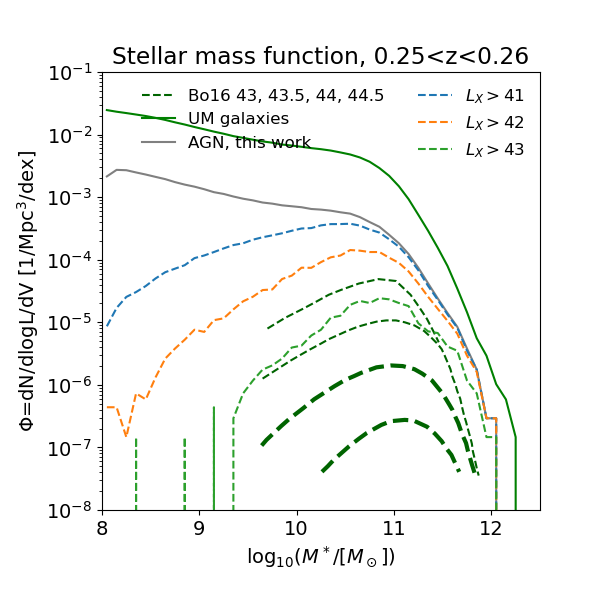
\includegraphics[width=0.95\linewidth]{figures_AGN/SMF_z025.png}
    %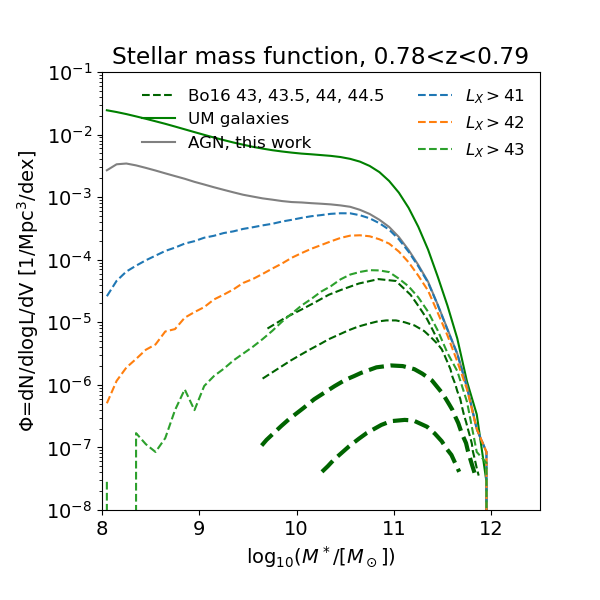
\includegraphics[width=0.45\linewidth]{figures_AGN/SMF_z075.png}
    %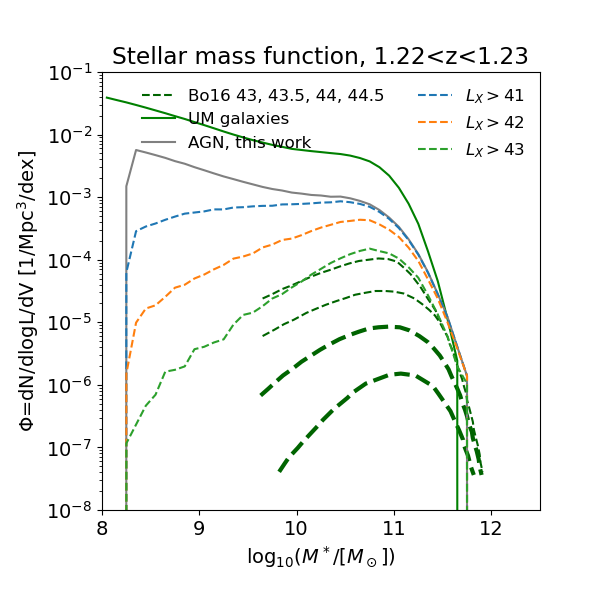
\includegraphics[width=0.45\linewidth]{figures_AGN/SMF_z125.png}
    \caption{Stellar mass function at z=0.25. 
    Number density of galaxies with a model active galactic nucleus as a function of stellar mass. 
    The model prediction is split (with colored dashes lines) for three hard X-ray (2-10 keV) luminosity thresholds (41, 42, 43) and the complete sample (grey).
    Observations (green dashes) from \citet[][Bo16]{BongiornoSchulzeMerloni_2016A&A...588A..78B} are shown for four luminosity thresholds 43, 43.5, 44, 44.5.
    The complete model galaxy population is shown with the solid green line.}
    \label{fig:AGN:SMF}
\end{figure}

This model starts from the hard X-ray luminosity function ans predicts via an obscuration model a soft X-ray luminosity function, shown in Fig. \ref{fig:AGN:softXLF}. 
The predicted unobscured soft X-ray luminosity function is in fair agreement with the measurements from \citet{HasingerMiyajiSchmidt2005A&A...441..417H}. 

\begin{figure}
    \centering
    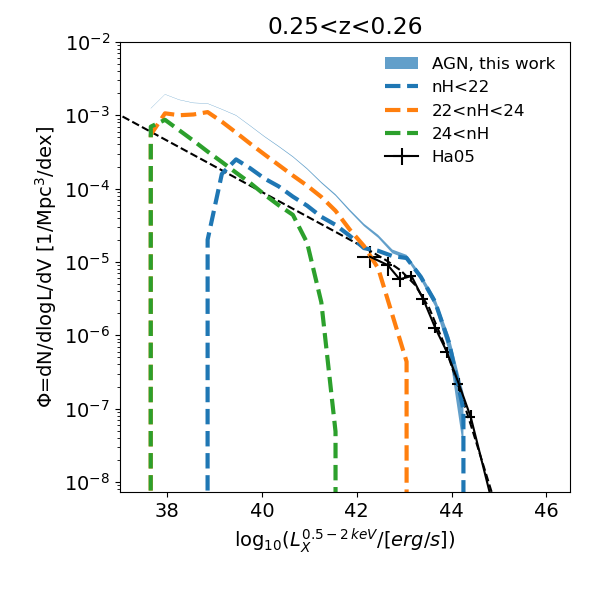
\includegraphics[width=0.95\linewidth]{figures_AGN/XLF_soft_z025.png}
    \caption{Soft X-ray luminosity function at z=0.25. 
    Number density of AGN as a function of soft X-ray luminosity. 
    The model prediction is split (with colored dashes lines) in three obscuration bins (delimited by 20, 22, 24, 26, unobscured, obscured, thick obscured) and the complete sample (blue).
    Observations (black crosses) and their best fit model (black dashes) from \citet[][Ha05]{HasingerMiyajiSchmidt2005A&A...441..417H} are shown. 
    The unobscured luminosity function (blue dashes) is in good agreement with observations.}
    \label{fig:AGN:softXLF}
\end{figure}

Finally, we find that the predicted number density of sources per square degree as a function of soft X-ray flux (logN-logS) is in fair agreement with observations \citep{MateosWarwickCarrera2008A&A...492...51M, GeorgakakisNandraLaird_2008MNRAS.388.1205G}, see Fig. \ref{fig:AGN:logNlogS}. 
The low number of very bright sources comes from the luminosity function used at low redshift. At the faint end, extending beyond redshift 4, provides a prediction closer to the observations.

\begin{figure}
    \centering
    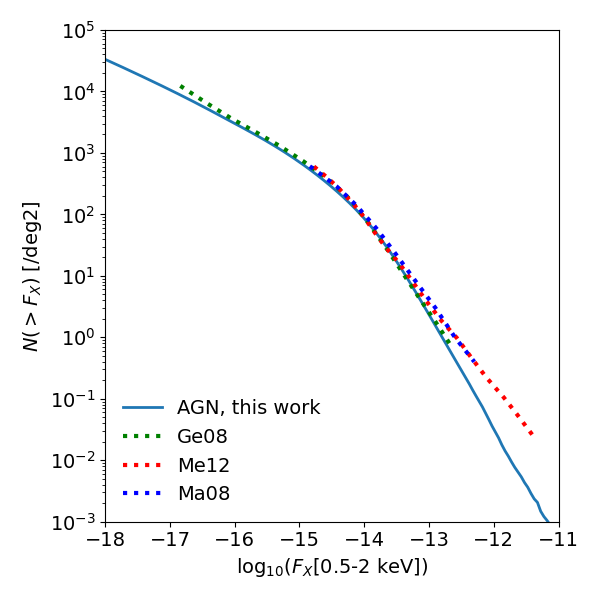
\includegraphics[width=0.95\linewidth]{figures_AGN/logNlogS_AGN_zupto4.png}
    \caption{logN-logS. Number density of sources per square degree as a function of soft X-ray flux with all AGN up to redshift 4. 
    Observations and their best fit model from \citet[][Ma08]{MateosWarwickCarrera2008A&A...492...51M} and  \citet[][Ge08]{GeorgakakisNandraLaird_2008MNRAS.388.1205G} are shown with dotted lines. 
    The model for the compilation presented by \citet[][Me12]{MerloniPredehlBecker_2012arXiv1209.3114M} is shown in red dots. 
    }
    \label{fig:AGN:logNlogS}
\end{figure}

This incarnation of the AGN model from \citet{ComparatMerloniSalvato_2019MNRAS.487.2005C}, using the Uchuu simulation and UniverseMachine galaxy model together with parameters from \citet{ComparatLuoMerloni_2023A&A...673A.122C}, seems to describe well to first order the AGN population (up to redshift of 4).  

\subsection*{Event generation}
To generate events, we limit the catalogs to sources brighter than $F^{\rm 0.5-2 keV}_X>10^{-16}$ erg cm$^{-2}$ s$^{-1}$. 
We tabulate X-ray spectra using the xspec models described in \citet{LiuMerloniComparat_2022A&A...661A..27L}. 
Events are then generated following an idealized eRASS:8 attitude file.

\clearpage
\section{Merging event files}

To characterize how sources are detected, different simulated experiments are needed. For each eROSITA field, we have five sets of event files: hot gas, active galactic nuclei, stars, particle background and true observed events. 

\subsection{Purity determination}

Purity is determined is a completely controlled environment. 
We merge all simulated event files, trimmed to match the exposure time of the real observations on the same field. 
We then run the source detection algorithm as in the observations and quantify the purity of the samples detected. 

\clearpage
\section{Cross-correlation benchmark}

We predict the intrinsic cross-correlation between central and satellite galaxies in narrow redshift bins and events in the 0.5-2 keV band coming from the hot gas, AGN and background model.
To avoid spurious correlation due to the box replication,
We filter events that come from sources located in the first replication of the simulation (with the src id) and add different number of background events to fill the required amount of events (the observed event density).


\clearpage
\section{Summary}

%\clearpage
\begin{acknowledgements}
---
\end{acknowledgements}

%%%%%%%%%%%%%%%%%%%% REFERENCES %%%%%%%%%%%%%%%%%%
\bibliographystyle{aa}
\bibliography{references}

%\clearpage
\appendix



\end{document}